%
% wuk.tex -- Wetter und Klima
%
% Einleitungskapitel, welches das Wetter- und Klimasystem der Erde in
% qualitiativer Form beschreibt
%
% (c) 2018 Prof Dr Andreas Müller, Hochschule Rapperswil
%
\chapter{Wetter und Klima}
\lhead{Wetter und Klima}
US Präsident Donald Trump war schon immer ein Klimaverweigerer, wie Tweets
aus der Zeit lange bevor er Präsident wurde:
\begin{center}
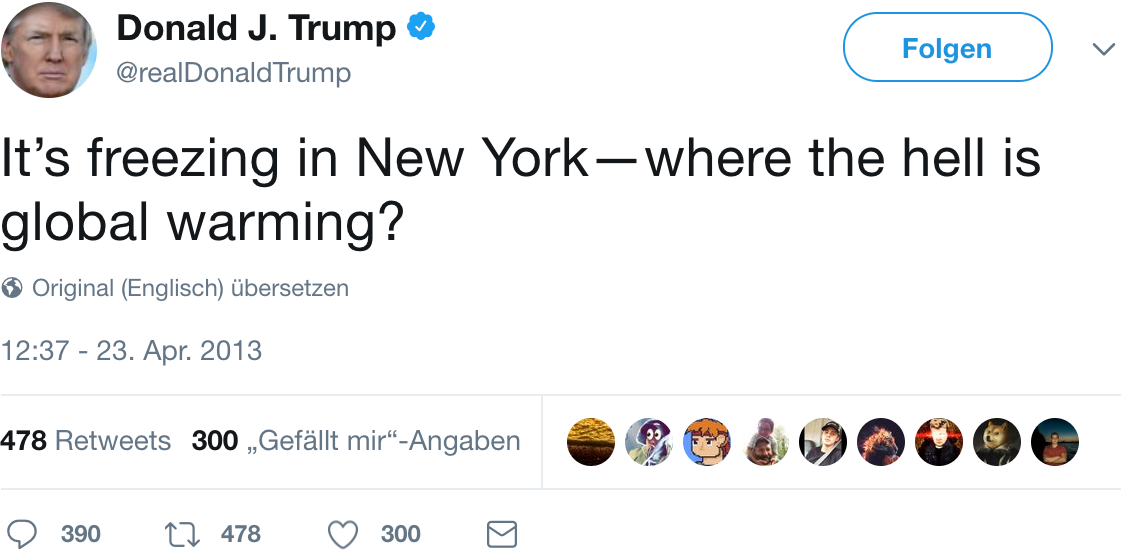
\includegraphics[width=\hsize]{chapters/1/trump.png}
\end{center}
Ganz offensichtlich versteht Trump den Unterschied zwischen Wetter und
Klima nicht.
Ziel dieses Kapitels ist, den Unterschied zwischen Wetter und Klima
zu klären.
Es ist allgemein bekannt, dass auch die besten Wetterprognosen im
günstigsten Fall für einige Tage zutreffen.
Daher soll in diesem Kapitel auch gezeigt werden, warm trotz dieser
Schwierigkeit das Klima sehr wohl langfristig modelliert und prognostiziert
werden kann.
Aus diesen Überlegungen wird auch klar, auf welche Aspekte des Klimasystems
sich ein Klima-Modell fokusieren muss, wenn eine langfristige Prognose
ermöglicht werden soll.

\section{Klima}
\rhead{Klima}
In der Wikipedia kann man die folgenden Definitionen für die Begriffe Wetter
und Klima finden:

\begin{definition}
Als {\em Wetter} bezeichnet man den
spürbaren, kurzfristigen Zustand der Atmosphäre (auch: messbarer
Zustand der Troposphäre) an einem bestimmten Ort der Erdoberfläche,
der unter anderem als Sonnenschein, Bewölkung, Regen, Wind, Hitze
oder Kälte in Erscheinung tritt.
\cite{skript:wetter}
\end{definition}

\begin{definition}
Das {\em Klima} steht als Begriff für die Gesamtheit aller meteorologischen
Vorgänge, die für die über Zeiträume von mindestens 30 Jahren
regelmässig wiederkehrenden durchschnittlichen Zustände der Erdatmosphäre
an einem Ort verantwortlich sind.
\cite{skript:klima}
\end{definition}

Was also Donald Trump in seinem Tweet beschrieben hat ist das Wetter.
Selbst wenn die Temperatur in New York unter den Gefrierpunkt fällt, 
heisst das nicht, dass die mittlere Temperatur in New York über mehrere
Jahre nicht doch ansteigen kann.
Tatsächlich bedeutet ``globale Erwärmung'' nicht, dass die mittlere
Temperatur an jedem Punkt der Erde zunehmen wird.
Im Gegenteil ist es durchaus möglich, dass zwar die mittlere Temperatur
der Erde ständig zunimmt, wie wir in den letzten Jahren auch messtechnisch
nachweisen konnten, dass aber auch die Temperaturunterschiede stark zunehmen,
so dass es am Ende an einzelnen Stelle der Erdoberfläche zu einer 
Abkühlung kommen kann.
Um dieser Komplexität Rechnung zu tragen, spricht man nicht mehr von
der ``globalen Erwärmung'', sondern vom Klimawandel.

Auch wenn das Wetter nur sehr eingeschränkt vorhersagen lässt,
bedeutet das noch lange nicht, dass das Klima nicht doch sehr
genau vorhergesagt werden kann.
Eine Analogie kann den Unterschied zwischen der Vorhersagbarkeit
von Wetter und Klima verdeutlichen.
Wenn man in einem Kochtopf Wasser zum Kochen bringt, stellt sich
eine unverrhersagbare chaotische Bewegung kleiner und grosser
Gasblasen ein.
Es ist unmöglich vorherzusagen, wann und wo sich die nächste Blase
bilden wird und welchen Weg sie an die Oberfläche des Wasser nehmen
wird.
Wenn wir aber nur die mittlere Temperatur betrachten, können wir
aus der Heizleistung der Kochplatte, der Masse und der spezifischen
Wärmekapazität des Wassers genau berechnen, welche Temperatur zu welcher
Zeit im Wasser herschen wird und wir können den Zeitpunkt exakt
vorhersagen, wann das Wasser zu sieden beginnt.
Die mittlere Temperatur des Wassers beschreibt das ``Klima''
in der Pfanne, die kleinräumigen und kurzfristigen Blasen und anderen
Turbulenzen beschreiben das ``Wetter''.

\section{Physikalische Eigenschaften des Klimasystems}
In diesem Abschnitt stellen wir die physikalischen Eigenschaften
aller wesentlicher Komponenten des Klimasystems zusammen.
Dabei geht es zunächst nur darum, die grundlegende Physik in 
Erinnerung zu rufen und die Naturgesetze, die die Wechselwirkungen
zwischen den Komponenten beschreiben.
Auf die Details der mathematischen Modellierung der zukünftigen
Veränderung dieser Grössen werden wir erst später eingehen.

\subsection{Wärme, Konvektion, Kondensation}
Die wohl wichtigste Klima-Grösse ist die Temperatur.
Sie drückt aus, wieviel Energie in Form von Wärme ein Körper enthält.

\subsubsection{Wärmekapazität}
Die spezifische Wärme $C$ gibt an, wie die innere Energie sich bei
einer Temperaturänderung $\Delta T$ verändert:
\[
\Delta E = C\cdot\Delta T.
\]
Der Körper speichert Energie in Form der thermischen Bewegung der
einzelnen Atome.
Schwerere Atome können bei gleicher Bewegungsgeschwindigkeit 
mehr Energie speichern.
Stoffe mit grösserer Dichte können mehr Atome und damit auch mehr
Wärmeenergie in einem kleineren Volumen unterbringen.
Die spezifische Wärmekapazität $c$ gibt an, welche Wärmekapazität
ein Kilogramm eines Stoffes hat.
Ein Körper der Masse $m$ hat also die Wärmekapazität $C=cm$.

\subsubsection{Wärmeleitung}
Herrschen in einem Körper Temperaturunterschiede, ist $T$ nicht mehr
nur eine konstante, sondern eine Funktion der Koordinaten und auch der
Zeit.
Temperaturunterschiede werden sich ausgleichen, indem Energie von
wärmeren zu kälteren Teilen des Körpers fliegt.
Dies geschieht umso schneller, je grösser die Unterschiede sind.
Die Wärmeleitungsgleichung
\begin{equation}
\frac{\partial T}{\partial t}
=
\kappa
\biggl(
\frac{\partial^2}{\partial x^2}
+
\frac{\partial^2}{\partial y^2}
+
\frac{\partial^2}{\partial z^2}
\biggr)
T
\label{skript:waermeleitung}
\end{equation}
beschreibt die Entwicklung der Funktion $T(x,y,z,t)$ an jedem
Ort des Raumes \cite{skript:waermeleitung}.
Der Koeffizient $\kappa$ ist eine Materialkonstante, die beschreibt,
wie schnell sich die Temperaturunterschiede ausgleichen können.
Ist $\kappa=0$, folgt $\partial T/\partial t=0$, die Temperatur 
ändert sich nicht, es findet keine Wärmeleitung statt.

Die rechte Seite von \eqref{skript:waermeleitung} kann mit dem
sogenannten Laplace-Operator gemäss der folgenden Definition 
geschrieben werden.

\begin{definition}
Der Operator
\[
\Delta
=
\frac{\partial^2}{\partial x^2}
+
\frac{\partial^2}{\partial y^2}
+
\frac{\partial^2}{\partial z^2}
\]
heisst der
{\em Laplace-Operator}.
\end{definition}

Die Wärmeleitungsgleichung erhält damit die Form
\begin{equation}
\frac{\partial T}{\partial t}
=
\kappa\Delta T.
\label{skript:waermeleitung2}
\end{equation}

\subsubsection{Konvektion}
Wärmeleitung kann Wärmeenergie nur vergleichsweise langsam transportieren.
Das einleitende Beispiel des Kochtopfs zeigt auch, wie ein effizienterer
Energietransport funktionieren kann.
In der Atmosphäre dehnt sich warme Luft aus.
Dank der geringeren Dichte können warme Luftblasen aufsteigen und damit
Wärme viel effizienter in die obere Atmosphäre transportieren
als dies mit Wärmeleitung möglich wäre.
Dieser Prozess heisst {\em Konvektion} \cite{skript:konvektion}.
\index{Konvektion}%

Wir wollen den Fall eines strömenden Mediums mathematisch etwas genauer
ausarbeiten.
Bewegt sich das Medium mit der Geschwindigkeit $\vec v$, dann ändert sich
die Temperatur des Mediums, welches sich über dem Punkt $P=(x,y,z)$
befindet.
Nach der Zeit $\Delta t$ befindet sich derjenige Teil des Mediums
über dem Punkt $P$, der sich vorher über dem Punkt $P-\Delta t\cdot\vec v$
befand.
Die Temperatur zur Zeit $t+\Delta t$ ist daher
$T(P,t+\Delta t)=T(P-\Delta t,t)$.
Die Temperaturänderung
\begin{align*}
T(P,t+\Delta t)
&=
T(P,t) + (T(P,t+\Delta t)-T(P,t))
=
T(P,t) + T(P-\vec v\Delta t, t)-T(P,t)
\\
\frac{
T(P,t+\Delta t)
-
T(P,t)
}{\Delta t}
&=
\frac{
T(P-\vec v\Delta t, t)-T(P,t)
}{\Delta t}.
\end{align*}
Beim Grenzübergang $\Delta t\to 0$ wird aus der linken Seite die
partielle Ableitung nach $t$.
Die rechte Seite kann mit Hilfe der Kettenregel berechnet weren.
Es wird
\begin{equation}
\frac{\partial T}{\partial t}
=
-
\frac{\partial T}{\partial x} v_x
-
\frac{\partial T}{\partial y} v_y
-
\frac{\partial T}{\partial z} v_z.
\label{skript:advektion1}
\end{equation}
Der Ausdruck auf der rechten Seite kann vektoriell mit der folgenden
Definition etwas eleganter geschrieben werden.

\begin{definition}
Der vektorielle Operator 
\[
\nabla
=
\begin{pmatrix}
\frac{\partial}{\partial x}\\
\frac{\partial}{\partial y}\\
\frac{\partial}{\partial z}
\end{pmatrix}
\]
heisst der {\em Nabla-Operator}.
Der Vektor
\[
\nabla f
=
\begin{pmatrix}
\frac{\partial f}{\partial x}\\
\frac{\partial f}{\partial y}\\
\frac{\partial f}{\partial z}
\end{pmatrix}
=
\operatorname{grad} f
\]
heisst der {\em Gradient} von $f$.
\end{definition}
\index{Gradient}%
\index{Nabla-Operator}%

Die Temperaturänderung in Folge der Strämung 
\eqref{skript:advektion1}
wird 
\begin{equation}
\frac{\partial T}{\partial t}
=
-\vec{v}\cdot\nabla T.
\label{skript:advektion2}
\end{equation}
\index{Advektion}%
Man nennt diese Temperaturänderung durch die Strömung auch
{\em Advektion}.
Die Wärmeleitungsgleichung kann damit zu einem umfassenderen
Modell
\begin{equation}
\frac{\partial T}{\partial t}
=
-\vec{v}\cdot\nabla T +\kappa\Delta T
\label{skript:waermeleitungadvektion}
\end{equation}
zusammengefasst werden.
Es ist geeignet für die Beschreibung sowohl der Atmosphäre wie auch des
Wärmeaustausches in den Ozeanen.

\subsubsection{Phasenübergänge}

\subsection{Strahlung}

\subsection{Erdrotation und Zirkulation}

\subsection{Periodische Einflüsse}

\section{Anforderungen an Klima-Modelle}



